\mfpicnumber{1}

\opengraphsfile{NonLinearInequalities}

\setcounter{footnote}{0}

\label{NonLinearInequalities}

With few exceptions, we have spent our time in this course graphing equations relating two variables.  In this section, we explore graphing inequalities relating two variables which  usually a two-dimensional \textit{region} in the plane instead of a one dimensional line or curve.\footnote{We have \textit{some} experience describing simple regions in the plane using inequalities from our work in Section \ref{Relations}.}  In our first example, we restrict our attention to looking at regions in the $xy$-plane bounded by equations which describe $y$ as a function of $x$.

\begin{ex}  \label{ineqgraphex01} $~$


\begin{enumerate}

\item Sketch the following sets of points in the $xy$-plane.


\begin{multicols}{2}

\begin{enumerate}

\item $R = \{ (x,y) \, | \,  y > |x| \}$

\item $S = \{ (x,y)  \, | \,   y \leq 6-x^2 \}$

\setcounter{HW}{\value{enumii}}

\end{enumerate}

\end{multicols}

\begin{enumerate}

\setcounter{enumii}{\value{HW}}
\item $T = \{ (x,y)  \, | \,   |x| < y \leq 6 -x^2 \}$

\end{enumerate}

\item  \label{describeregionex} Find a set builder description for each of the following regions described below:

\begin{enumerate}

\item \label{parabolalineregionex} The region graphed below:

\begin{center}

\begin{mfpic}[20]{-4}{4}{-1}{5}
\fillcolor[gray]{.7}
\gfill \btwnfcn{-1,2,0.1}{x**2}{x+2}
\axes
\tlabel[cc](4,-0.5){\scriptsize $x$}
\tlabel[cc](0.5,5){\scriptsize $y$}
\gclear \tlabelrect(0,3){\scriptsize $y=x+2$ \vphantom{ $\frac{x^2}{x^2}$} }
%\tlabel[cc](-2,1){\scriptsize $(-1,1)$}
%\tlabel[cc](2.75,4){\scriptsize $(2,4)$}
\tlabel[cc](2.5,2){\scriptsize $y=x^2$}
\xmarks{-3 step 1 until 3}
\ymarks{1, 2, 4}
\tcaption{\scriptsize The region  $R$}
\scriptsize
\tlpointsep{4pt}
\axislabels {x}{{$-3 \hspace{7pt}$} -3,{$-2 \hspace{7pt}$} -2,{$-1 \hspace{7pt}$} -1,{$1$} 1,{$2$} 2,{$3$} 3}
\axislabels {y}{{$1$} 1,{$2$} 2,{$4$} 4}
\normalsize 
\gfill \btwnfcn{0.5,2,0.1}{x**2}{x+2}
\penwd{1.25pt}
\function{-1,2,0.1}{x**2}
\function{-1,2,0.1}{x+2}
\point[4pt]{(-1,1), (2,4)}
\end{mfpic}

\end{center}

\item  The region $S$ between the graphs\footnote{sometimes written as `the region bounded by the graphs' \ldots} of $f(x) = x^3-3x$ and $g(x) = x$.


\end{enumerate}


\end{enumerate}

{\bf Solution.}  

\begin{enumerate}

\item 

\begin{enumerate}

\item  The set $R$ consists of all points $(x,y)$ whose $y$-coordinate is greater than $|x|$.  If we graph $y=|x|$, we get the familiar `$\vee$' shape with vertex at $(0,0)$.  Hence, in order for an ordered pair $(x,y)$ to satisfy  $y > |x|$,  the point $(x,y)$ must be \textit{above} the graph of $y = |x|$.  

Since the inequality here, $y > |x|$ is strict, we use a dashed line with which to indicate the graph of  $y=|x|$ and shade the region above, or `inside,' the `$\vee$' as shown below on the left.  

Note that one way to check our answer is to choose points both inside and outside the shaded region to verify the inequality either holds or it doesn't, respectively.

\item  Using the same reasoning as above we note a point $(x,y)$ is in  $S$ if its  $y$-coordinate is less than or equal to the $y$-coordinate on the parabola $y=6-x^2$.  Hence, we graph the points  \textit{below} the parabola ($y < 6-x^2$) along with the points \textit{on} the parabola ($y=6-x^2$)  below on the right.

\begin{center}

\begin{tabular}{m{3in}m{3in}}

\begin{mfpic}[15]{-7}{7}{-2}{7}
\fillcolor[gray]{.7}
\gfill \btwnfcn{-6.75,0,0.1}{-x+0.01}{6.75}
\gfill \btwnfcn{0,6.75,0.1}{x+0.01}{6.75}
\axes
\tlabel[cc](7,-0.5){\scriptsize $x$}
\tlabel[cc](0.5,7){\scriptsize $y$}
\xmarks{-6 step 1 until 6}
\ymarks{-1 step 1 until 6}
\tcaption{\scriptsize $R = \{ (x,y) : y > |x| \}$}
\scriptsize
\tlpointsep{4pt}
\axislabels {x}{{$-6 \hspace{7pt}$} -6,{$-5 \hspace{7pt}$} -5,{$-4 \hspace{7pt}$} -4,{$-3 \hspace{7pt}$} -3,{$-2 \hspace{7pt}$} -2,{$-1 \hspace{7pt}$} -1,{$1$} 1,{$2$} 2,{$3$} 3,{$4$} 4,{$5$} 5,{$6$} 6}
\axislabels {y}{{$-1$} -1,{$1$} 1,{$2$} 2,{$3$} 3,{$4$} 4,{$5$} 5,{$6$} 6}
\normalsize 
\penwd{1.25pt}
\arrow \reverse \arrow \dashed \polyline{(-7,7),(0,0),(7,7)}
\end{mfpic} \hspace{2.5in} & 

\begin{mfpic}[15]{-7}{7}{-2}{7}
\fillcolor[gray]{.7}
\gfill \btwnfcn{-2.82,2.82,0.1}{6-(x**2)}{-1.75}
\axes
\tlabel[cc](7,-0.5){\scriptsize $x$}
\tlabel[cc](0.5,7){\scriptsize $y$}
\xmarks{-6 step 1 until 6}
\ymarks{-1 step 1 until 6}
\tcaption{\scriptsize $S = \{ (x,y) :  y \leq 2-x^2 \}$}
\scriptsize
\tlpointsep{4pt}
\axislabels {x}{{$-6 \hspace{7pt}$} -6,{$-5 \hspace{7pt}$} -5,{$-4 \hspace{7pt}$} -4,{$-3 \hspace{7pt}$} -3,{$-2 \hspace{7pt}$} -2,{$-1 \hspace{7pt}$} -1,{$1$} 1,{$2$} 2,{$3$} 3,{$4$} 4,{$5$} 5,{$6$} 6}
\axislabels {y}{{$-1$} -1,{$1$} 1,{$2$} 2,{$3$} 3,{$4$} 4,{$5$} 5,{$6$} 6.25}
\normalsize 
\penwd{1.25pt}
\arrow \reverse \arrow \function{-2.82,2.82,0.1}{6-(x**2)}

\end{mfpic} \\

\end{tabular}

\end{center}

\item For a point $(x,y)$ to be in $T$, the $y$-coordinate must satisfy $|x| < y \leq 6-x^2$ which means it must belong to both $R$ and $S$.\footnote{Said differently, $T$ is the set-theoretic intersection of $R$ and $S$, $T = R \cap S$ as described in \ref{AppSetTheory}.} Thus we shade the region \textit{between} $y=|x|$ and $y=6-x^2$, keeping those points on the parabola, but not the points on $y=|x|$.  

To get an accurate graph, we need to find where these two graphs intersect, so we set $|x| = 6-x^2$.  Using the techniques discussed in Sections \ref{AbsoluteValueFunctions} and \ref{QuadraticFunctions}, we find  $x=-2,2$.  To find the associated $y$-coordinates of the intersection points, we substitute $x= \pm 2$ into either $y = |x|$ or $y = 6-x^2$ (or both, to check!)  In both cases, we find the associated $y$-coordinate  to be $2$, so the intersection points are $(-2,2)$ and $(2,2)$.  On our graph, however, these are the location of `holes' owing to the strictness of the inequality $y > |x|$.

\begin{center}

\begin{mfpic}[15]{-7}{7}{-2}{7}
\fillcolor[gray]{.7}
\gfill \btwnfcn{-2,0,0.1}{-x+0.01}{6-(x**2)}
\gfill \btwnfcn{0,2,0.1}{x+0.01}{6-(x**2)}
\axes
\tlabel[cc](7,-0.5){\scriptsize $x$}
\tlabel[cc](0.5,7){\scriptsize $y$}
\tlabel[cc](3,2){\scriptsize $(2,2)$}
\tlabel[cc](-3.25,2){\scriptsize $(-2,2)$}
\xmarks{-6 step 1 until 6}
\ymarks{-1 step 1 until 6}
\tcaption{\scriptsize $T = \{ (x,y) : |x| < y \leq 6 -x^2 \}$}
\scriptsize
\tlpointsep{4pt}
\axislabels {x}{{$-6 \hspace{7pt}$} -6,{$-5 \hspace{7pt}$} -5,{$-4 \hspace{7pt}$} -4,{$-3 \hspace{7pt}$} -3,{$-2 \hspace{7pt}$} -2,{$-1 \hspace{7pt}$} -1,{$1$} 1,{$2$} 2,{$3$} 3,{$4$} 4,{$5$} 5,{$6$} 6}
\axislabels {y}{{$-1$} -1,{$1$} 1,{$2$} 2,{$3$} 3,{$4$} 4,{$5$} 5,{$6$} 6.25}
\normalsize 
\penwd{1.25pt}
\function{-2,2,0.1}{6-(x**2)}
\dashed \polyline{(-2,2),(0,0),(2,2)}
\pointfillfalse
\point[4pt]{(-2,2), (2,2)}

\end{mfpic}

\end{center}

\end{enumerate}


\item

\begin{enumerate}

\item  Verbally, we may describe $R$ as the region \textit{between} the graphs of $y = x^2$ and $y = x+2$.  More specifically, $R$ is the set of points \textit{above} (or on) the parabola  $y=x^2$ but \textit{below} (or on) the line $y = x+2$.  That is, for the points $(x,y)$ in $R$, we have $x^2 \leq y \leq x+2$.  

To find the restrictions on $x$, we find the intersection of the graphs.  Solving $x^2 = x+2$ gives $x = -1$ and $x = 2$.  Hence, to be in $R$, points $(x,y)$ need to satisfy $-1 \leq x \leq 2$.  Hence, one way to describe $R$ is $R = \{ (x,y)  \, | \,  -1 \leq x \leq 2, \,  x^2 \leq y \leq x+2 \}$.

While this answer is correct, the fact that the line and the parabola intersect only twice producing only \textit{one} region where the inequality  $x^2 \leq y \leq x+2$ is true,  we may shorten our description of $R$ to just  $R = \{ (x,y)  \, | \,   x^2 \leq y \leq x+2 \}$.  

\item  Since we are given a verbal description of $S$, we first sketch the graph to get a sense of the geometric situation.  To graph $f(x) = x^3-3x$, we use what we learned in Section \ref{GraphsofPolynomials}:  end behavior, behavior near the $x$-intercepts, and symmetry.  The graph of $g(x) = x$ is a line with slope $1$ through the origin.

Graphing both of these functions on the same pair of axes, we see three intersection points.  Solving $f(x) = g(x)$, that is $x^3-3x = x$ gives $x = 0$ and  $x = \pm 2$.  These solutions correspond to the intersection points $(-2,-2)$, $(0,0)$, and $(2,2)$.    $S$ is described as the region `\textit{between}' these graphs, so we shade between the graphs accordingly.



\begin{center}

\begin{mfpic}[15]{-5}{5}{-5}{5}
\fillcolor[gray]{.7}
\gfill \btwnfcn{-2,0,0.1}{(x**3)-(3*x)}{x}
\gfill \btwnfcn{0,2,0.1}{x}{(x**3)-(3*x)}
\axes
\tlabel[cc](5,-0.5){\scriptsize $x$}
\tlabel[cc](0.5,5){\scriptsize $y$}
\tlabel[cc](3,2){\scriptsize $(2,2)$}
\tlabel[cc](-3.5, -2){\scriptsize $(-2,-2)$}
\xmarks{-4 step 1 until 4}
\ymarks{-4 step 1 until 4}
\tcaption{\scriptsize Graphing $f(x) = x^3-3x$ and $g(x) = x$}
\scriptsize
\tlpointsep{4pt}
\axislabels {x}{{$-4 \hspace{7pt}$} -4,{$-3 \hspace{7pt}$} -3,{$-2 \hspace{7pt}$} -2,{$-1 \hspace{7pt}$} -1,{$1$} 1,{$2$} 2,{$3$} 3,{$4$} 4}
\axislabels {y}{{$-4$} -4,{$-3$} -3,{$-2$} -2,{$-1$} -1,{$2$} 2,{$3$} 3,{$4$} 4}
\normalsize 
\penwd{1.25pt}
\arrow \reverse \arrow \function{-2.2,2.2,0.1}{(x**3)-(3*x)}
\arrow \reverse \arrow \polyline{(-4.5,-4.5),(4.5, 4.5)}
\point[4pt]{(-2,-2), (0,0), (2,2)}

\end{mfpic}

\end{center}

From the graph, we see that for $-2 < x < 0$,  the graph of $f$ is above the graph of $g$.  Algebraically, this means that for all $x$ with $-2 \leq x \leq 0$, $f(x) \geq g(x)$ or $x^3-3x \geq x$.  At $x=0$, the situation changes and we have $f(x) \leq g(x)$ or $x^3-3x \leq x$ for $0 \leq x \leq 2$.  One to describe $S$ is to describe each of these pieces and take their set theoretic union. 

We first consider the piece for $-2 \leq x \leq 0$. Unlike the previous problem, we cannot completely describe this region in terms of the $y$-values since there are \textit{two} regions where $x \leq y \leq x^3-3x$ is true:  one where $-2 \leq x \leq 0$ (the one we want) and one here $x \geq 2$ (which we don't want.) Hence, we describe this first piece as $ \{ (x,y) \, | \, -2 \leq x \leq 0, \, x \leq y \leq x^3-3x \}$.  Following this methodology for the second piece, we obtain the complete description for $S$ below: 

    \[ S = \{ (x,y) \, | \, -2 \leq x \leq 0, \, x \leq y \leq x^3-3x \} \cup\{ (x,y) \, | \, 0 \leq x \leq 2, \, x^3-3x \leq y \leq x \}. \]


\qed

\end{enumerate}

\end{enumerate}

\end{ex}

A few remarks about Example \ref{ineqgraphex01} are in order.  First note that each of the regions presented here can be views as graphs of relations as described in Section \ref{Relations}.  Moreover, there are many ways to describe a region so our answers to number \ref{describeregionex} above are by no means unique.

In particular, our solution $R = \{ (x,y)  \, | \,  -1 \leq x \leq 2, \,  x^2 \leq y \leq x+2 \}$ to number  \ref{parabolalineregionex} can be visualized as `filling up' the region $R$ from the bottom curve, $y = x^2$ to the top curve, $y = x+2$ as $x$ runs from the leftmost extent of the region at $x = -1$ to the rightmost extent at $x = 2$ as indicated below. The notion that each $x$ determines where to start and stop filling the region is a consequence of us viewing the bounding curves as functions of $x$.  That is, for each $x$, we can determine the lower boundary of the region, $y = x^2$ and the upper boundary of the region, $y = x+2$.

\begin{center}

\begin{tabular}{ccc}

\begin{mfpic}[20]{-4}{4}{-1}{5}
\axes
\tlabel[cc](4,-0.5){\scriptsize $x$}
\tlabel[cc](0.5,5){\scriptsize $y$}
\tlabel[cc](-2,1){\scriptsize $(-1,1)$}
\tlabel[cc](2.75,4){\scriptsize $(2,4)$}
\xmarks{-3 step 1 until 3}
\ymarks{1, 2, 3, 4}
\tcaption{\scriptsize `Filling up'  $R$ from bottom to top.}
\scriptsize
\tlpointsep{4pt}
\axislabels {x}{{$-3 \hspace{7pt}$} -3,{$-2 \hspace{7pt}$} -2,{$-1 \hspace{7pt}$} -1,{$1$} 1,{$2$} 2,{$3$} 3}
\axislabels {y}{ {$2$} 2, {$3$} 3,{$4$} 4}
\normalsize 
\arrow \polyline{ (-0.75, 0.5625), (-0.75, 1.15)}
\arrow \polyline{ (-0.5, 0.25), (-0.5, 1.4)}
\arrow \polyline{ (-0.25, 0.0625), (-0.25, 1.65)}
\arrow \polyline{ (0, 0), (0,1.8)}
\arrow \polyline{ (0.25, 0.0625), (0.25, 2.15)}
\arrow \polyline{ (0.5, 0.25), (0.5,2.4)}
\arrow \polyline{ (0.75, 0.5625), (0.75, 2.65)}
\arrow \polyline{ (1, 1), (1,2.9)}
\arrow \polyline{ (1.25, 1.5625), (1.25,3.15)}
\arrow \polyline{ (1.5, 2.25), (1.5,3.4)}
\arrow \polyline{ (1.75,3.0625), (1.75,3.65)}
\penwd{1.25pt}
\function{-1,2,0.1}{x**2}
\function{-1,2,0.1}{x+2}
\point[4pt]{(-1,1), (2,4)}
\end{mfpic}

&

$\xrightarrow{\hspace{0.5in}}$

&

\begin{mfpic}[20]{-4}{4}{-1}{5}
\fillcolor[gray]{.7}
\gfill \btwnfcn{-1,2,0.1}{x**2}{x+2}
\axes
\tlabel[cc](4,-0.5){\scriptsize $x$}
\tlabel[cc](0.5,5){\scriptsize $y$}
\gclear \tlabelrect(0,3){\scriptsize $y=x+2$ \vphantom{ $\frac{x^2}{x^2}$} }
%\tlabel[cc](-2,1){\scriptsize $(-1,1)$}
%\tlabel[cc](2.75,4){\scriptsize $(2,4)$}
\tlabel[cc](2.5,2){\scriptsize $y=x^2$}
\xmarks{-3 step 1 until 3}
\ymarks{1, 2, 4}
\tcaption{\scriptsize The region $R$.}
\scriptsize
\tlpointsep{4pt}
\axislabels {x}{{$-3 \hspace{7pt}$} -3,{$-2 \hspace{7pt}$} -2,{$-1 \hspace{7pt}$} -1,{$1$} 1,{$2$} 2,{$3$} 3}
\axislabels {y}{{$1$} 1,{$2$} 2,{$4$} 4}
\normalsize 
\gfill \btwnfcn{0.5,2,0.1}{x**2}{x+2}
\penwd{1.25pt}
\function{-1,2,0.1}{x**2}
\function{-1,2,0.1}{x+2}
\point[4pt]{(-1,1), (2,4)}
\end{mfpic} \\

\end{tabular}

\end{center}

There are times in Calculus where it may be convenient to describe the region $R$ as filling up left-to-right as $y$ varies from the bottom most extent, $y = 0$ to the top most extent, $y = 4$.  In this case, we need to describe the bounding curves as functions of $y$.  To that end, we solve $y = x+2$ and $y = x^2$ for $x$ and get three functions of $y$:  $x = y-2$, $x = \sqrt{y}$ and $x = -\sqrt{y}$ as labeled below.

\begin{tabular}{ccc}

\begin{mfpic}[20]{-4}{4}{-1}{5}
\axes
\tlabel[cc](4,-0.5){\scriptsize $x$}
\tlabel[cc](0.5,5){\scriptsize $y$}
\tlabel[cc](-2,1){\scriptsize $(-1,1)$}
\tlabel[cc](0.5,-0.5){\scriptsize $(0,0)$}
\tlabel[cc](2.75,4){\scriptsize $(2,4)$}
\xmarks{-3 step 1 until 3}
\ymarks{2, 3, 4}
\tcaption{\scriptsize `Filling up'  $R$ from left to right.}
\scriptsize
\tlpointsep{4pt}
\axislabels {x}{{$-3 \hspace{7pt}$} -3,{$-2 \hspace{7pt}$} -2,{$-1 \hspace{7pt}$} -1,{$2$} 2,{$3$} 3}
\axislabels {y}{ {$2$} 2, {$3$} 3,{$4$} 4}
\normalsize 
\arrow \polyline{ (-0.5, 0.25), (0.4, 0.25)}
\arrow \polyline{ (-0.7, 0.5), (0.6, 0.5)}
\arrow \polyline{ (-0.86, 0.75), (0.76, 0.75)}
\dotted  \polyline{ (-1, 1), (1, 1)}
\arrow \polyline{ (-0.75, 1.25), (1.01, 1.25)}
\arrow \polyline{ (-0.5, 1.5), (1.12, 1.5)}
\arrow \polyline{ (-0.25, 1.75), (1.22, 1.75)}
\arrow \polyline{ (0, 2), (1.31, 2)}
\arrow \polyline{ (0.25, 2.25), (1.4, 2.25)}
\arrow \polyline{ (0.5, 2.5), (1.48, 2.5)}
\arrow \polyline{ (0.75, 2.75), (1.55, 2.75)}
\arrow \polyline{ (1, 3), (1.63, 3)}
\arrow \polyline{ (1.25, 3.25), (1.70, 3.25)}
\arrow \polyline{ (1.5, 3.5), (1.77, 3.5)}
\penwd{1.25pt}
\function{-1,2,0.1}{x**2}
\function{-1,2,0.1}{x+2}
\point[4pt]{(-1,1), (2,4), (0,0)}
\end{mfpic}

&

$\xrightarrow{\hspace{0.5in}}$

&

\begin{mfpic}[20]{-4}{4}{-1}{5}
\fillcolor[gray]{.7}
\gfill \btwnfcn{-1,2,0.1}{x**2}{x+2}
\axes
\tlabel[cc](4,-0.5){\scriptsize $x$}
\tlabel[cc](0.5,5){\scriptsize $y$}
\tlabel[cc](1.75,1){\scriptsize $y=1$}
\tlabel[cc](2.5,2){\scriptsize $x = \sqrt{y}$}
\tlabel[cc](1.5,0.5){\scriptsize $x = \sqrt{y}$}
\tlabel[cc](-2,0.5){\scriptsize $x = - \sqrt{y}$}
\gclear \tlabelrect(0,3){\scriptsize $x=y-2$ \vphantom{ $\frac{x^2}{x^2}$} }
%\tlabel[cc](-2,1){\scriptsize $(-1,1)$}
%\tlabel[cc](2.75,4){\scriptsize $(2,4)$}
\xmarks{-3 step 1 until 3}
\ymarks{1, 2, 4}
\tcaption{\scriptsize The region  $R$}
\scriptsize
\tlpointsep{4pt}
\axislabels {x}{{$-3 \hspace{7pt}$} -3,{$-2 \hspace{7pt}$} -2,{$-1 \hspace{7pt}$} -1,{$1$} 1,{$2$} 2,{$3$} 3}
\axislabels {y}{{$2$} 2,{$4$} 4}
\normalsize 
\gfill \btwnfcn{0.5,2,0.1}{x**2}{x+2}
\polyline{(-1,1), (1,1)}
\penwd{1.25pt}
\function{-1,2,0.1}{x**2}
\function{-1,2,0.1}{x+2}
\point[4pt]{(-1,1), (2,4), (1,1), (0,0)}
\end{mfpic} \\

\end{tabular}


Based on the diagram, we see we need to describe $R$ as \textit{two} pieces.  The first piece being bounded on the left by $x = -\sqrt{y}$ and on the right $x = \sqrt{y}$  from $y = 0$ to $y=1$, and the second piece bounded on the left by $x = y-2$ and on the right by $x= \sqrt{y}$ from $y = 1$ to $y = 4$.  That is,

    \[ R = \{ (x,y) \, | \, 0 \leq y \leq 1, \, -\sqrt{y} \leq x \leq \sqrt{y} \} \cup\{ (x,y) \, | \, 1 \leq y \leq 4, \, y-2 \leq x \leq \sqrt{y} \}. \]

\newpage

Not all regions in the plane are best described using functions of $x$ or $y$.\footnote{See Section \ref{PolarGraphs} for instance!} Suppose, for instance,  we wish to sketch the region $\{ (x,y) \, | \,  x^2 < 4 - y^2. \}$  Algebraically, we wish to plot all points $(x,y)$ for which the inequality $x^2<4 - y^2$ is true.  One way to proceed is to mimic the `sign diagram' routine we use for solving nonlinear inequalities in one variable:   rewrite the inequality so as to obtain $0$ on one side of the inequality, find the zeros of the non-zero side, choose test values determined by the zeros, and record our solution.

First, we gather all of the terms on one side and leave a $0$ on the other:  $x^2 + y^2 -4 < 0$.  Next, we find the zeros of the left hand side, that is, where is $x^2 + y^2 - 4 = 0$.  Rewriting, we get $x^2+y^2 = 4$ which describes the circle of radius $2$ centered at the origin.  In other words, instead of obtaining a few \textit{numbers} which divide the real number \textit{line} into \textit{intervals}, we get an equation of a \textit{curve}, in this case, a circle, which divides the \textit{plane} into two \textit{regions} - the `inside' and `outside' of the circle.  

Just like we used test \textit{values} to determine whether or not an interval belongs to the solution of the inequality, we use test \textit{points} in the each of the regions to see which of these belong to our solution set.\footnote{The theory behind why all this works is, surprisingly, the same theory which guarantees that sign diagrams work the way they do - continuity and the Intermediate Value Theorem - but in this case, applied to functions of more than one variable.}  We choose $(0,0)$ to represent the region inside the circle and $(0,3)$ to represent the points outside of the circle. When we substitute $(0,0)$ into $x^2 + y^2 -4 < 0$, we get $-4 < 4$ which is true.  This means $(0,0)$ and all the other points inside the circle are part of the solution.  On the other hand, when we substitute $(0,3)$ into the same inequality, we get $5 < 0$ which is false.  This means $(0,3)$ along with all other points outside the circle are not part of the solution.  What about points on the circle itself?  Choosing a point on the circle, say $(0,2)$, we get $0 < 0$, which means the circle itself does not satisfy the inequality.\footnote{Another way to see this is that points on the circle satisfy $x^2 + y^2 - 4 = 0$, so they do not satisfy $x^2 + y^2 - 4 < 0$.}  As a result, we leave the circle dashed in the final diagram. 

\begin{center}

\begin{mfpic}[25]{-3}{3}{-3}{3}
\fillcolor[gray]{.7}
\gfill \btwnfcn{-1.99,1.99,0.1}{0-sqrt(4-x**2)}{sqrt(4-x**2)}
\axes
\tlabel[cc](3,-0.5){\scriptsize $x$}
\tlabel[cc](0.5,3){\scriptsize $y$}
\tlabel[cc](0.5,2.25){\scriptsize $2$}
\tlabel[cc](0.5,-2.25){\scriptsize $-2$}
\xmarks{-2,-1,1,2}
\ymarks{-2,-1,1,2}
\tlpointsep{4pt}
\axislabels {x}{{\scriptsize $-2 \hspace{15pt}$} -2, {\scriptsize $\hspace{7pt} 2$} 2}
\penwd{1.25pt}
\dashed \circle{(0,0),2.01}
\end{mfpic}

The solution to $x^2 < 4 - y^2$

\end{center}

We put this technique to good use in the following example.

\newpage

\begin{ex} \label{nonlinearineqex}   $~$  

\begin{enumerate}

\item  Sketch the following regions in the $xy$-plane:

\begin{enumerate}

\item $R = \{ (x,y) \, | \, y^2 - 4 \leq x < y+2 \}$

\item  The solution to: $\left\{\begin{array}{rcr}  x^2 +y^2 & \geq & 4 \\ x^2 - 2x + y^2 - 2y & \leq & 0 \\ \end{array} \right.$

\end{enumerate}

\item  Find a set builder description for the region between the Unit Circle and the graph of  $x^2+y^2 = 16$.

\end{enumerate}

{\bf Solution.}  

\begin{enumerate}

\item \begin{enumerate}

\item  The inequality $y^2 - 4 \leq x < y+2$ is a compound inequality which translates as $y^2 - 4 \leq x$ \textit{and} $x < y+2$. Hence, our approach is to solve each inequality separately and take the set theoretic intersection to determine the region which satisfies both inequalities.  

Starting with $y^2 - 4 \leq x$, we rewrite this as $y^2 - x - 4 \leq 0$ and set about graphing $y^2 - x - 4 = 0$.  Since only one variable is squared, we know this equation describes a parabola.   Rewriting in  standard form, we get $y^2 = x+4$, so the vertex is $(-4,0)$ and the parabola opens to the right.  

Using the test points $(-5,0)$ and $(0,0)$, we find that the solution to the inequality includes the region to the \textit{right} of, or `inside', the parabola.  The points on the parabola itself are also part of the solution, owing to the `equality' in the `inequality.'  (We could also check a point on the parabola such as $(-4,0)$ satisfies the inequality.) 

Turning our attention to $x < y+2$, we first rewrite this as $x - y - 2 < 0$ and focus our attention on $x-y-2 = 0$.   Rewriting, we have the line $y = x-2$ and using the test points $(0,0)$ and $(0,-4)$, we find points in the region \textit{above} the line satisfy the inequality.   (Owing to the strictness of the inequality, the points on the line itself do not.)\footnote{We could also have rewritten $x<y+2$ as $y > x-2$ directly and sketched the region as explained in Example \ref{ineqgraphex01}.}

We see that these two regions do overlap but to make the graph more precise, we seek the intersection of these two curves.  That is, we need to solve the system of nonlinear equations

\[\left\{\begin{array}{lrcr}  (E1) & y^2 & = & x + 4 \\ (E2) & y & = & x - 2 \\ \end{array} \right.\]

Solving $E1$ for $x$, we get $x = y^2 - 4$.  Substituting this into $E2$ gives $y = y^2 - 4 - 2$, or $y^2-y-6 = 0$.  We find $y = -2$ and $y=3$ and since $x = y^2-4$, we get that the graphs intersect at $(0,-2)$ and $(5,3)$.  Putting all of this together, we get our final answer below.

\[ \begin{array}{ccc}

\begin{mfpic}[10]{-6}{6}{-4}{4}
\fillcolor[gray]{.7}
\gfill \btwnfcn{-4,5.5,0.1}{0-sqrt(x+4)}{sqrt(x+4)}
\axes
\tlabel[cc](6,-0.5){\scriptsize $x$}
\tlabel[cc](0.5,4){\scriptsize $y$}
\xmarks{-5,-4,-3,-2,-1,1,2,3,4,5}
\ymarks{-3,-2,-1,1,2,3}
\tlpointsep{4pt}
\axislabels {x}{{\scriptsize $-5 \hspace{7pt}$} -5}
\axislabels {y}{{\scriptsize $-3$} -3,{\scriptsize $3$} 3}
\penwd{1.25pt}
\arrow \reverse \arrow \parafcn{-3.16,3.16,0.1}{(t^2-4,t)}
\end{mfpic}

&

\hspace{.25in}

\begin{mfpic}[10]{-6}{6}{-4}{4}
\fillcolor[gray]{.7}
\gfill \btwnfcn{-2,5.5,0.1}{x-2}{3.5}
\gfill \btwnfcn{-6,-2,0.1}{-4}{3.5}

\axes
\tlabel[cc](6,-0.5){\scriptsize $x$}
\tlabel[cc](0.5,4){\scriptsize $y$}
\xmarks{-5,-4,-3,-2,-1,1,2,3,4,5}
\ymarks{-3,-2,-1,1,2,3}
\tlpointsep{4pt}
\axislabels {x}{{\scriptsize $2$} 2, {\scriptsize $3$} 3,{\scriptsize $4$} 4,{\scriptsize $5$} 5}
\penwd{1.25pt}
\dashed \polyline{(-2,-4), (5.5,3.5)}
\end{mfpic} 

&

\hspace{.25in}

\begin{mfpic}[10]{-6}{6}{-4}{4}
\fillcolor[gray]{.7}
\gfill \btwnfcn{-4,0,0.1}{0-sqrt(x+4)}{sqrt(x+4)}
\gfill \btwnfcn{0,5,0.1}{x-2}{sqrt(x+4)}
\axes
\tlabel[cc](6,-0.5){\scriptsize $x$}
\tlabel[cc](0.5,4){\scriptsize $y$}
\tlabel[cc](2, -2){\scriptsize $(0,-2)$}
\tlabel[cc](5,4){\scriptsize $(5,3)$}
\xmarks{-5,-4,-3,-2,-1,1,2,3,4,5}
\ymarks{-3,-1,1,2,3}
\tlpointsep{4pt}
\axislabels {x}{{\scriptsize $-5 \hspace{7pt}$} -5, {\scriptsize $2$} 2, {\scriptsize $3$} 3,{\scriptsize $4$} 4,{\scriptsize $5$} 5}
\penwd{1.25pt}
\parafcn{-2,3,0.1}{(t^2-4,t)}
\dashed \polyline{(0,-2), (5,3)}
\pointfillfalse
\point[4pt]{(0,-2), (5,3)}
\end{mfpic} \\

y^2 - 4 \leq x & \hspace{.25in}  x < y+2 & \hspace{.25in} y^2 - 4 \leq x < y+2 \\

\end{array} \]

\item  Like any system, our solution to this problem requires us to graph the points $(x,y)$ which satisfy \textit{both} inequalities.  To do this, we solve each inequality separately and take the set theoretic intersection of the solution sets.  

We begin with the inequality $x^2 + y^2 \geq 4$ which we rewrite as $x^2+y^2 - 4 \geq 0$.  The points which satisfy $x^2 + y^2 - 4 = 0$ form the circle $x^2+y^2 = 4$.   Using test points $(0,0)$, $(0,2)$,  and $(0,3)$ we find that our solution comprises the region \textit{outside} the circle along with the circle itself.  

Moving to  $x^2 - 2x + y^2 - 2y \leq 0$, we start with $x^2 - 2x + y^2 - 2y = 0$.  Completing the squares, we obtain $(x-1)^2 + (y-1)^2 = 2$, which is a circle centered at $(1,1)$ with a radius of $\sqrt{2}$.  

Choosing $(1,1)$ to represent the inside of the circle,  $(0,0)$ as a point on the circle, and $(1,3)$ as a point outside of the circle, we find that the solution to the inequality is the inside of the circle, including the circle itself.  

Our final answer, then, consists of the points on or outside of the circle $x^2 + y^2 = 4$ which lie on or inside the circle $(x-1)^2+(y-1)^2 = 2$.  To produce the most accurate graph, we need to find where these circles intersect.  To that end, we solve the system

\[\left\{\begin{array}{lrcr}  (E1) & x^2 + y^2 & = & 4 \\ (E2) & x^2 - 2x + y^2 - 2y & = & 0 \\ \end{array} \right.\]

We can eliminate both the $x^2$ and $y^2$ by replacing $E2$ with $-E1 + E2$.  Doing so produces $-2x - 2y = -4$.  Solving  for $y$ gives $y = 2-x$.  Substituting this into $E1$ gives $x^2 + (2-x)^2 = 4$ which simplifies to $x^2 + 4-4x+x^2 = 4$ or $2x^2 - 4x = 0$.  Factoring yields $2x(x-2)$ which gives $x=0$ or $x=2$.  Substituting these values into $y=2-x$ gives the points $(0,2)$ and $(2,0)$.  The intermediate graphs and final solution are below.


\[ \begin{array}{ccc}

\begin{mfpic}[15]{-4}{4}{-4}{4}
\fillcolor[gray]{.7}
\gfill \btwnfcn{-3.5,3.5,0.1}{-3.5}{3.5}
\gclear \circle{(0,0),2}
\axes
\tlabel[cc](4,-0.5){\scriptsize $x$}
\tlabel[cc](0.5,4){\scriptsize $y$}
\xmarks{-3,-2,-1,1,2,3}
\ymarks{-3,-2,-1,1,2,3}
\tlpointsep{4pt}
\axislabels {x}{{\scriptsize $1$} 1 }
\axislabels {y}{{\scriptsize $-1$} -1,{\scriptsize $1$} 1}
\penwd{1.25pt}
\circle{(0,0),2}
\end{mfpic}

&

\hspace{.25in}

\begin{mfpic}[15]{-4}{4}{-4}{4}
\fillcolor[gray]{.7}
\gfill \circle{(1,1),1.414}
\axes
\tlabel[cc](4,-0.5){\scriptsize $x$}
\tlabel[cc](0.5,4){\scriptsize $y$}
\xmarks{-3,-2,-1,1,2,3}
\ymarks{-3,-2,-1,1,2,3}
\tlpointsep{4pt}
\axislabels {x}{{\scriptsize $-3 \hspace{7pt}$} -3,{\scriptsize $-2 \hspace{7pt}$} -2,{\scriptsize $-1 \hspace{7pt}$} -1, {\scriptsize $\hspace{7pt} 2$} 2}
\axislabels {y}{{\scriptsize $-3$} -3,{\scriptsize $-2$} -2,{\scriptsize $-1$} -1,{\scriptsize $2$} 2,{\scriptsize $3$} 3}
\penwd{1.25pt}
\circle{(1,1),1.414}
\end{mfpic}

&

\hspace{.25in}

\begin{mfpic}[15]{-4}{4}{-4}{4}
\fillcolor[gray]{.7}
\penwd{1.25pt}
\gfill \circle{(1,1),1.414}
\circle{(1,1),1.414}
\gclear \circle{(0,0),2}
\arc[s]{(2,0),(0,2),90} 
\penwd{0.5pt}
\axes
\tlabel[cc](4,-0.5){\scriptsize $x$}
\tlabel[cc](0.5,4){\scriptsize $y$}
\xmarks{-3,-2,-1,1,2,3}
\ymarks{-3,-2,-1,1,2,3}
\tlpointsep{4pt}
\axislabels {x}{{\scriptsize $-3 \hspace{7pt}$} -3,{\scriptsize $-2 \hspace{7pt}$} -2,{\scriptsize $-1 \hspace{7pt}$} -1}
\axislabels {y}{{\scriptsize $-3$} -3,{\scriptsize $-2$} -2,{\scriptsize $-1$} -1,{\scriptsize $3$} 3}
\point[4pt]{(0,2), (2,0)}
\tlabel[cc](-1, 2){\scriptsize $(0,2)$}
\tlabel[cc](2,-0.5){\scriptsize $(2,0)$}
\end{mfpic} \\
x^2+y^2 \geq 4 & \hspace{.25in} x^2 - 2x + y^2 - 2y \leq 0  & \hspace{.25in} \text{Solution to the system.} \\

\end{array} \]

\end{enumerate}

\item We first recall the Unit Circle is the circle centered at the origin with radius $1$ and hence is described algebraically by the equation $x^2+y^2 = 1$.  The equation $x^2+y^2 = 16$ describes a circle centered at the origin with radius $4$.  Hence, the `region between' these two circles indicates we want is \textit{outside} the Unit Circle but \textit{inside} the circle $x^2+y^2 = 16$. 

Based on our experience from the earlier problems, we know points outside the Unit Circle satisfy $x^2+y^2 > 1$ whereas the points inside the circle $x^2+y^2 = 16$ satisfy $x^2+y^2<16$.  Hence, the points we seek satisfy \textit{both} inequalities, so our solution is $\{ (x,y) \, | \, 1 < x^2+y^2 < 16 \}$.  \qed

\end{enumerate}

\end{ex}

We close this section with a follow-up to Example \ref{circuitex} in Section \ref{MatMethods}.  Recall in the circuit diagrammed below, we have two batteries with source voltages $V\!B_{\text{\scriptsize$1$}}$ and $V\!B_{\text{\scriptsize$2$}}$, measured in volts $V$, along with six resistors with resistances $R_{\text{\scriptsize$1$}}$ through $R_{\text{\scriptsize$6$}}$, measured in kiloohms, $k\Omega$.Recall if we think of electrons flowing through the circuit, we can think of the voltage sources as providing the `push' which makes the electrons move, the resistors as obstacles for the electrons to overcome, and the mesh current as a net rate of flow of electrons around the indicated loops.


\centerline{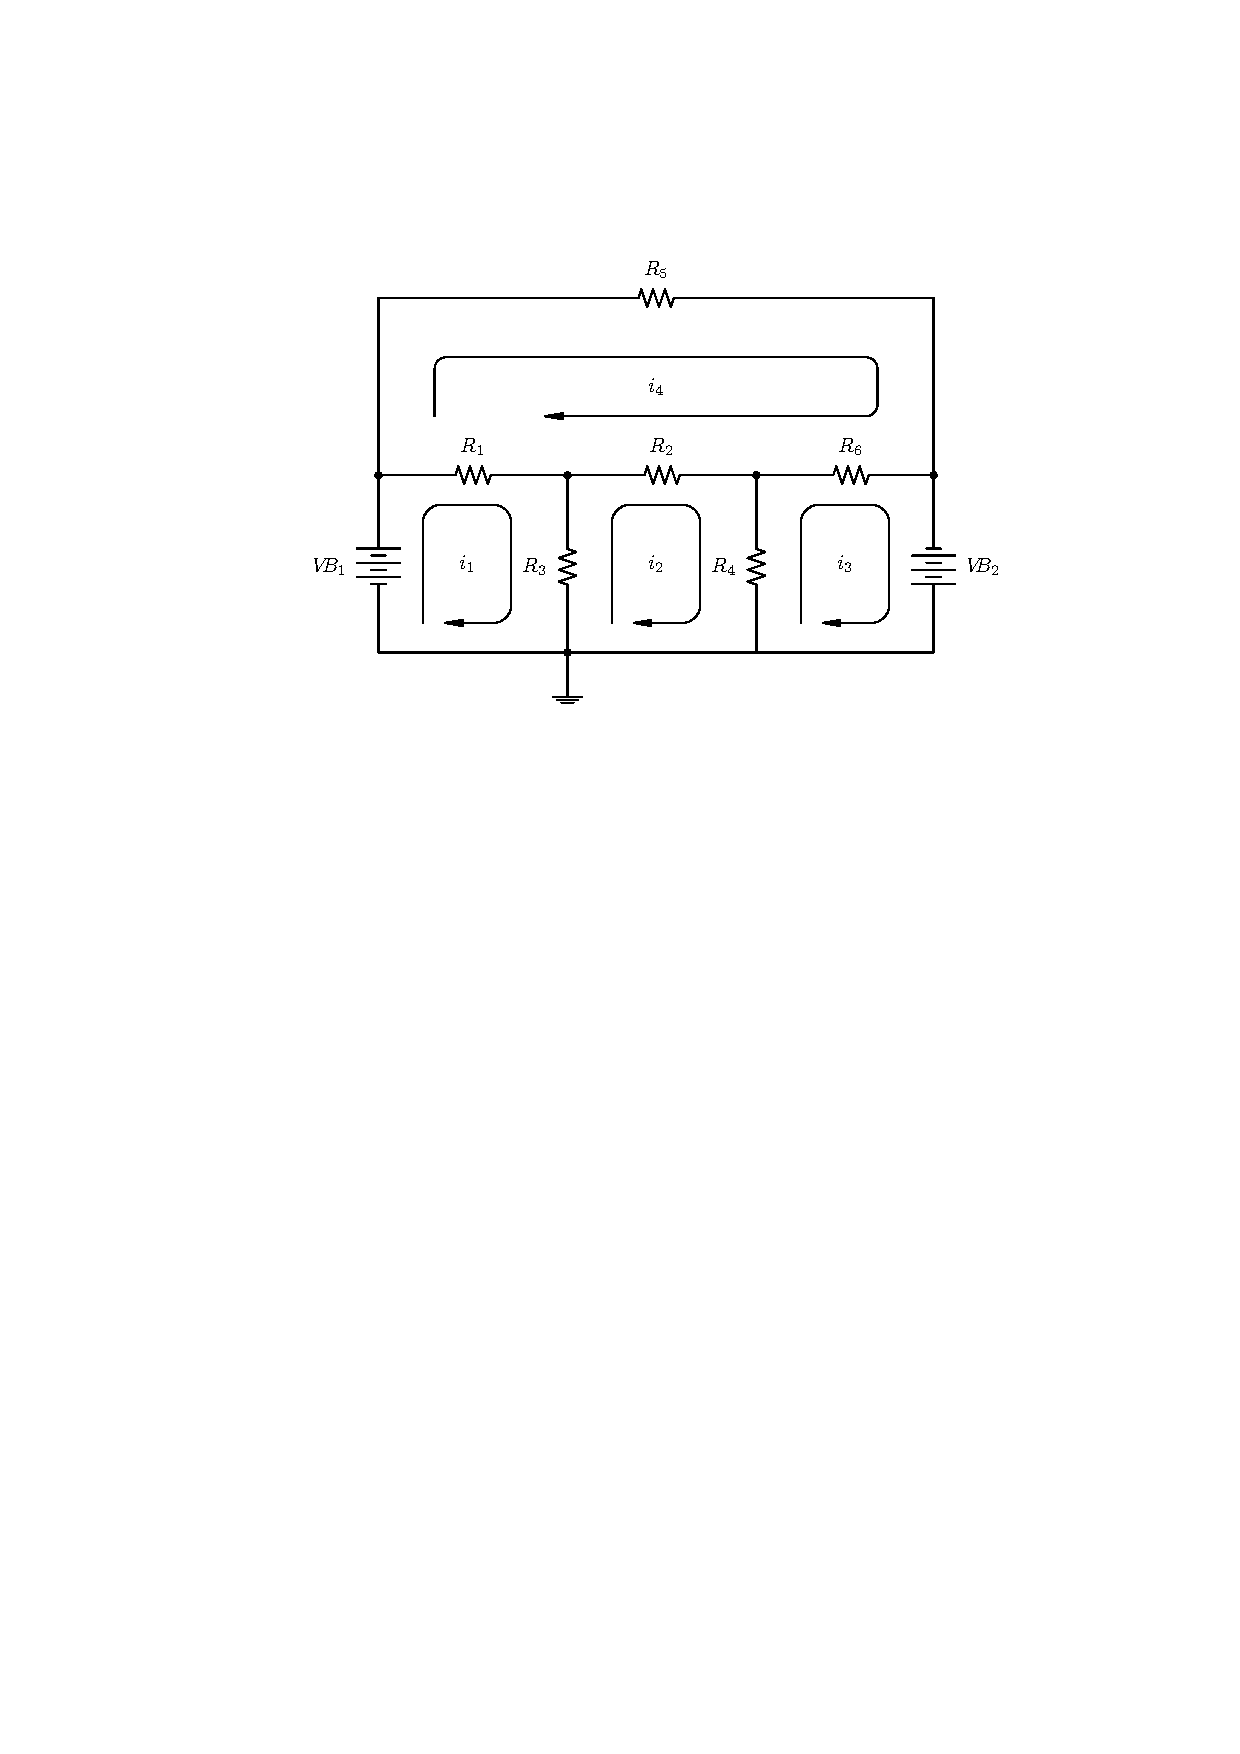
\includegraphics{./NonLinearInequalitiesGraphics/CircuitDiagram01.pdf}}

Using \href{http://en.wikipedia.org/wiki/Ohm's_law}{\underline{Ohm's Law}} \index{Ohm's Law} \index{Kirchhoff's Voltage Law} and \href{http://en.wikipedia.org/wiki/Kirchhoff's_circuit_laws}{\underline{Kirchhoff's Voltage Law}}, we can relate the voltage supplied to the circuit by the two batteries to the voltage drops across the six resistors in order to find the four `mesh' currents: $i_{\text{\scriptsize$1$}}$, $i_{\text{\scriptsize$2$}}$, $i_{\text{\scriptsize$3$}}$ and $i_{\text{\scriptsize$4$}}$, measured in milliamps, $mA$. This gives rise to the following system of linear equations:

\[ \left\{ \begin{array}{rcl} \left(R_{\text{\scriptsize$1$}} + R_{\text{\scriptsize$3$}}\right)i_{\text{\scriptsize$1$}} - R_{\text{\scriptsize$3$}}i_{\text{\scriptsize$2$}} - R_{\text{\scriptsize$1$}}i_{\text{\scriptsize$4$}} & = & V\!B_{\text{\scriptsize$1$}} \\
-R_{\text{\scriptsize$3$}}i_{\text{\scriptsize$1$}} + \left(R_{\text{\scriptsize$2$}} + R_{\text{\scriptsize$3$}} + R_{\text{\scriptsize$4$}}\right)i_{\text{\scriptsize$2$}} - R_{\text{\scriptsize$4$}}i_{\text{\scriptsize$3$}} - R_{\text{\scriptsize$2$}}i_{\text{\scriptsize$4$}} & = & 0 \\
-R_{\text{\scriptsize$4$}}i_{\text{\scriptsize$2$}} + \left(R_{\text{\scriptsize$4$}} + R_{\text{\scriptsize$6$}}\right)i_{\text{\scriptsize$3$}} - R_{\text{\scriptsize$6$}}i_{\text{\scriptsize$4$}} & = & -V\!B_{\text{\scriptsize$2$}} \\
-R_{\text{\scriptsize$1$}}i_{\text{\scriptsize$1$}} - R_{\text{\scriptsize$2$}}i_{\text{\scriptsize$2$}} - R_{\text{\scriptsize$6$}}i_{\text{\scriptsize$3$}} + \left(R_{\text{\scriptsize$1$}} + R_{\text{\scriptsize$2$}} + R_{\text{\scriptsize$5$}} + R_{\text{\scriptsize$6$}}\right)i_{\text{\scriptsize$4$}} & = & 0 \\  \end{array} \right.\]

In Example \ref{circuitex}, we found that under the assumptions $V\!B_{\text{\scriptsize$1$}} = 10 V$, $V\!B_{\text{\scriptsize$2$}} = 5 V$, and all  the resistances are all $1 k\Omega$, the mesh currents worked out to be $i_{\text{\scriptsize$1$}} = 10.625 \, \, mA$, $i_{\text{\scriptsize$2$}} = 6.25 \, \, mA$, $i_{\text{\scriptsize$3$}} = 3.125 \, \, mA$, and $i_{\text{\scriptsize$4$}} = 5 \, \, mA$. 

 In our final example, we assume  $V\!B_{\text{\scriptsize$1$}} = 10 V$ and  $V\!B_{\text{\scriptsize$2$}} = 5 V$  and work to find what combination of resistances would combine to produce these mesh currents.
 

\begin{ex}  \label{circuitex02}  For the circuit described above, if $V\!B_{\text{\scriptsize$1$}} = 10 V$ and $V\!B_{\text{\scriptsize$2$}} = 5 V$, find the possible combinations of resistances which yield the currents  $i_{\text{\scriptsize$1$}} = 10.625 \, \, mA$, $i_{\text{\scriptsize$2$}} = 6.25 \, \, mA$, $i_{\text{\scriptsize$3$}} = 3.125 \, \, mA$, and $i_{\text{\scriptsize$4$}} = 5 \, \, mA$.

\newpage

{\bf Solution.}

We begin by substituting the known values of the currents into the system of equations.  We get:

\[ \left\{ \begin{array}{rcr} 5.625R_{\text{\scriptsize$1$}} + 4.375R_{\text{\scriptsize$3$}}& = & 10 \\
1.25R_{\text{\scriptsize$2$}} - 4.375R_{\text{\scriptsize$3$}} + 3.125R_{\text{\scriptsize$4$}}& = & 0 \\
-3.125R_{\text{\scriptsize$4$}} - 1.875R_{\text{\scriptsize$6$}} & = & -5 \\
-5.625R_{\text{\scriptsize$1$}} - 1.25R_{\text{\scriptsize$2$}} + 5R_{\text{\scriptsize$5$}} + 1.875R_{\text{\scriptsize$6$}} & = & 0 \\  \end{array} \right.\]

The coefficient matrix for this system is $4 \times 6$ (4 equations with 6 unknowns) and is therefore not invertible.  We do know, however, this system is consistent, since setting all the resistance values equal to $1$ corresponds to our situation Example \ref{circuitex}.  This means we have an underdetermined consistent system which is necessarily dependent.  To solve this system, we encode it into an augmented matrix

\[ \left[ \begin{array}{rrrrrr|r} 
5.25 & 0 & 4.375 & 0 & \hphantom{1.2}0 & 0 & 10 \\ 
0 & 1.25 & -4.375 & 3.125 & 0 & 0 & 0 \\ 
0 & 0 & 0 & -3.125 & 0 & -1.875 & -5 \\
 -5.625 & -1.25 & 0 & 0 & 5 & 1.875 & 0 \\ 
 \end{array} \right] \]

A graphing utility gives the reduced-row echelon form of the matrix as:

\[\left[ \begin{array}{rrrrrr|r} 
1 & \hphantom{-1.}0 & 0.\overline{7} & \hphantom{-1.}0 & \hphantom{-1.}0 & 0 & 1.\overline{7} \\ 
0 & 1 & -3.5           & 0 & 0 & -1.5 & -4 \\ 
0 & 0 & 0              & 1 & 0 & 0.6 & 1.6 \\ 
0 & 0 & 0              & 0 & 1 & 0 & 1 \\ 
\end{array} \right] \]

from which we obtain the system:

\[ \left\{ \begin{array}{rcr} R_{\text{\scriptsize$1$}} + 0.\overline{7}R_{\text{\scriptsize$3$}}& = & 1.\overline{7} \\
R_{\text{\scriptsize$2$}} - 3.5R_{\text{\scriptsize$3$}} - 1.5R_{\text{\scriptsize$6$}}& = & -4 \\
R_{\text{\scriptsize$4$}} + 0.6R_{\text{\scriptsize$6$}} & = & 1.6 \\
R_{\text{\scriptsize$5$}}& = & 1 \\  \end{array} \right.\]

We can solve for $R_{\text{\scriptsize$1$}}$, $R_{\text{\scriptsize$2$}}$, $R_{\text{\scriptsize$4$}}$ and $R_{\text{\scriptsize$5$}}$ leaving $R_{\text{\scriptsize$3$}}$ and $R_{\text{\scriptsize$6$}}$ as free variables.  Labeling $R_{\text{\scriptsize$3$}} = s$ and $R_{\text{\scriptsize$6$}} = t$, we have $R_{\text{\scriptsize$1$}} = - 0.\overline{7}s + 1.\overline{7}$, $R_{\text{\scriptsize$2$}} = 3.5s + 1.5t - 4$, $R_{\text{\scriptsize$4$}} = -0.6t + 1.6$ and $R_{\text{\scriptsize$5$}} = 1$.  

Since resistance values are always positive, we need to restrict our values of $s$ and $t$.  We know $R_{\text{\scriptsize$3$}} = s > 0$ and when we combine that with $R_{\text{\scriptsize$1$}} = - 0.\overline{7}s + 1.\overline{7} >0$, we get $0 < s < 2.\overline{285714}$.  Similarly, $R_{\text{\scriptsize$6$}} = t > 0$ and with $R_{\text{\scriptsize$4$}} = -0.6t + 1.6 > 0$, we find $0 < t <2.\overline{6}$. 

 In order visualize the inequality $R_{\text{\scriptsize$2$}} = 3.5s + 1.5t - 4 > 0$, we graph the line $3.5s + 1.5t - 4 =0$ on the $ts$-plane below on the left and shade accordingly.    Imposing the additional conditions $0 < s < 2.\overline{285714}$ and $0 < t <2.\overline{6}$, we find our values of $s$ and $t$ restricted to the region $R$ graphed below on the right.  
 
 

\[ \begin{array}{cc}

\begin{mfpic}[20]{-3}{5}{-2}{4}
\fillcolor[gray]{.7}
\gfill \btwnfcn{-2.25,4.75,0.1}{(4.1-1.5*x)/3.5}{3.5}
\axes
\penwd{1.25pt}
\dashed \arrow \reverse \arrow \function{-2.5,5,0.1}{(4-1.5*x)/3.5}
\xmarks{-2,-1,1,2,3,4}
\ymarks{-1,1,2,3}
\tlabel(5,-0.5){\scriptsize $t$}
\tlabel(0.25,4){\scriptsize $s$}
\tcaption{ \scriptsize The region where $3.5s+1.5t-4> 0$}
\tlpointsep{5pt}
\axislabels {x}{{\scriptsize $-2 \hspace{7pt}$} -2,  {\scriptsize $-1 \hspace{7pt}$} -1, {\scriptsize $1$} 1, {\scriptsize $2$} 2, {\scriptsize $4$} 4}
\axislabels {y}{{\scriptsize $-1$} -1, {\scriptsize $1$} 1, {\scriptsize $2$} 2, {\scriptsize $3$} 3}
\end{mfpic}

&

\begin{mfpic}[20]{-3}{5}{-2}{4}
\fillcolor[gray]{.7}
\gfill \btwnfcn{0,2.6666,0.1}{(4.1-1.5*x)/3.5}{2.2857}
\penwd{1.25pt}
\arrow \dashed \polyline{(0,-2), (0,4)}
\arrow \polyline{(-3,0),(5,0)}
\dashed \polyline{(-1.5,2.2857),(4,2.2857)}
\dashed \polyline{(2.6666,-1),(2.6666,3)}
\dashed \arrow \reverse \arrow \function{-2.5,5,0.1}{(4-1.5*x)/3.5}
\xmarks{-2,-1,1,2,3,4}
\ymarks{-1,1,2,3}
\tlabel(5,-0.5){\scriptsize $t$}
\tlabel(0.25,4){\scriptsize $s$}
\tlabel[cc](2.6666,-1.75){\scriptsize $t =2.\overline{6}$}
\tlabel[cc](4.75,2){\scriptsize $s =2.\overline{285714}$}
\tcaption{ \scriptsize The region $R$ for our parameters $s$ and $t$.}
\tlpointsep{5pt}
\axislabels {x}{{\scriptsize $-2 \hspace{7pt}$} -2,  {\scriptsize $-1 \hspace{7pt}$} -1, {\scriptsize $1$} 1, {\scriptsize $2$} 2, {\scriptsize $4$} 4}
\axislabels {y}{{\scriptsize $-1$} -1, {\scriptsize $1$} 1, {\scriptsize $2$} 2, {\scriptsize $3$} 3}
\end{mfpic}

\end{array} \]

 Hence,  our final answer is:    
 
 
 \[ \left\{ \begin{array}{rcr}
R_{\text{\scriptsize$1$}} & = & - 0.\overline{7}s + 1.\overline{7}\\
R_{\text{\scriptsize$2$}}  & = &  3.5s + 1.5t - 4 \\
R_{\text{\scriptsize$4$}}  & = &  -0.6t + 1.6 \\
R_{\text{\scriptsize$5$}} & = & 1, \\  \end{array} \right.\]
 
where $s$ and $t$ are pulled from the region $R = \left\{ (s,t) \, | \,  0 < s < 2.\overline{285714}, \, \,  0 < t < 2.\overline{6}, \, \, 3.5s+1.5t-4 > 0\right\}$.  

The reader is encouraged to check that the solution presented in Example \ref{circuitex}, namely all resistance values equal to $1$, corresponds to a pair $(s,t)$ in this region. \qed

\end{ex}

\newpage

\subsection{Exercises}

\label{ExercisesforNonLinearInequalities}

In Exercises \ref{nonlinearsysineqfirst} - \ref{nonlinearsysineqlast}, sketch the solution to each system of nonlinear inequalities in the plane.


\begin{multicols}{2}
\begin{enumerate}
%\setcounter{enumi}{\value{HW}}


\item $\left\{\begin{array}{rcr}  x^{2} - y^{2} & \leq & 1 \\ x^{2} + 4y^{2} & \geq & 4  \end{array} \right.$ \label{nonlinearsysineqfirst}
\item $\left\{\begin{array}{rcr}  x^{2} + y^{2} & < & 25 \\ x^{2} + (y - 3)^{2} & \geq & 10  \end{array} \right.$

\setcounter{HW}{\value{enumi}}
\end{enumerate}
\end{multicols}

\begin{multicols}{2}
\begin{enumerate}
\setcounter{enumi}{\value{HW}}

\item $\left\{\begin{array}{rcr}  (x - 2)^{2} + y^{2} & < & 1 \\ x^{2} + 4y^{2} & < & 4  \end{array} \right.$
\item $\left\{\begin{array}{rcr}  y & > & 10x - x^{2} \\ y & < & x^{3} + 8  \end{array} \right.$

\setcounter{HW}{\value{enumi}}
\end{enumerate}
\end{multicols}

\begin{multicols}{2}
\begin{enumerate}
\setcounter{enumi}{\value{HW}}

\item $\left\{\begin{array}{rcr}  x + 2y^{2} & > & 2 \\ x^{2} + 4y^{2} & \leq & 4  \end{array} \right.$
\item $\left\{\begin{array}{rcr}  x^{2} + y^{2} & \geq & 25 \\ y - x & \leq & 1  \end{array} \right.$ \label{nonlinearsysineqlast}

\setcounter{HW}{\value{enumi}}
\end{enumerate}
\end{multicols}

%\begin{enumerate}
%\setcounter{enumi}{\value{HW}}

\newpage

\subsection{Answers}

\begin{multicols}{2}
\begin{enumerate}
%\setcounter{enumi}{\value{HW}}

\item $\left\{\begin{array}{rcr}  x^{2} - y^{2} & \leq & 1 \\ x^{2} + 4y^{2} & \geq & 4  \end{array} \right.$ \\

\begin{mfpic}[15]{-3}{3}{-3}{3}
\fillcolor[gray]{.7}
\gfill \rect{(-2.8,-2.8),(2.8,2.8)}
\gclear \btwnfcn{-3,-1,0.1}{sqrt((x**2) - 1)}{-sqrt((x**2) - 1)}
\gclear \btwnfcn{1,3,0.1}{sqrt((x**2) - 1)}{-sqrt((x**2) - 1)}
\gclear \btwnfcn{-2,2,0.1}{sqrt(1 - ((x**2)/4))}{-sqrt(1 - ((x**2)/4))}
\function{-1.2649,1.2649,0.1}{sqrt(1 - ((x**2)/4))}
\function{-1.2649,1.2649,0.1}{-sqrt(1 - ((x**2)/4))}
\arrow \reverse \function{-3,-1.2649,0.1}{sqrt((x**2) - 1)}
\arrow \reverse \function{-3,-1.2649,0.1}{-sqrt((x**2) - 1)}
\arrow \function{1.2649,3,0.1}{sqrt((x**2) - 1)}
\arrow \function{1.2649,3,0.1}{-sqrt((x**2) - 1)}
\axes
\tlabel[cc](3,-0.5){\scriptsize $x$}
\tlabel[cc](0.5,3){\scriptsize $y$}
\xmarks{-2,-1,1,2}
\ymarks{-2,-1,1,2}
\tlpointsep{4pt}
\tiny
\axislabels {x}{{$-2 \hspace{7pt}$} -2, {$-1 \hspace{7pt}$} -1, {$1$} 1, {$2$} 2}
\axislabels {y}{{$-2$} -2, {$-1$} -1, {$1$} 1, {$2$} 2}
\normalsize
\end{mfpic}

\vfill

\columnbreak

\item $\left\{\begin{array}{rcr}  x^{2} + y^{2} & < & 25 \\ x^{2} + (y - 3)^{2} & \geq & 10  \end{array} \right.$\\

\begin{mfpic}[10]{-6}{6}{-6}{5}
\fillcolor[gray]{.7}
\gfill \circle{(0,0),5}
\dashed \circle{(0,0),5}
\gclear \circle{(0,3),3.16228}
\arc[t]{(-3,4),(0,-0.166228),(3,4)}
\gclear \circle{(3,4),0.15}
\circle{(3,4),0.15}
\gclear \circle{(-3,4),0.15}
\circle{(-3,4),0.15}
\axes
\tlabel[cc](6,-0.5){\scriptsize $x$}
\tlabel[cc](0.5,5){\scriptsize $y$}
\xmarks{-5 step 1 until 5}
\ymarks{-5 step 1 until 4}
\tlpointsep{4pt}
\tiny
\axislabels {x}{{$-5 \hspace{7pt}$} -5, {$-4 \hspace{7pt}$} -4, {$-3 \hspace{7pt}$} -3, {$-2 \hspace{7pt}$} -2, {$-1 \hspace{7pt}$} -1, {$1$} 1, {$2$} 2, {$3$} 3, {$4$} 4, {$5$} 5}
\axislabels {y}{{$-5$} -5, {$-4$} -4, {$-3$} -3, {$-2$} -2, {$-1$} -1, {$1$} 1, {$2$} 2, {$3$} 3, {$4$} 4}
\normalsize
\end{mfpic}

\setcounter{HW}{\value{enumi}}
\end{enumerate}
\end{multicols}

\begin{multicols}{2}
\begin{enumerate}
\setcounter{enumi}{\value{HW}}

\item $\left\{\begin{array}{rcr}  (x - 2)^{2} + y^{2} & < & 1 \\ x^{2} + 4y^{2} & < & 4  \end{array} \right.$ \\

\begin{mfpic}[30]{0}{2.75}{-1.5}{1.5}
\fillcolor[gray]{.7}
\gfill \circle{(2,0),1}
\gclear \btwnfcn{1.3333,2,0.1}{sqrt(1 - ((x**2)/4))}{sqrt(1 - ((x - 2)**2))}
\gclear \btwnfcn{1.3333,2,0.1}{-sqrt(1 - ((x**2)/4))}{-sqrt(1 - ((x - 2)**2))}
\gclear \btwnfcn{2,3,0.1}{-sqrt(1 - ((x - 2)**2))}{sqrt(1 - ((x - 2)**2))}
\gclear \rect{(2.5,-1),(3,1)}
\drawcolor{white} \arc[t]{(1.3333,-0.745356),(3,0),(1.3333,0.745356)}
\drawcolor{white} \polyline{(2,-1),(2,1)}
\drawcolor{black}
\dashed \arc[t]{(1.3333,-0.745356),(1,0),(1.3333,0.745356)}
\dashed \parafcn{-0.84107,0.84107,0.1}{(2*cos(t),sin(t))}

\axes
\tlabel[cc](2.75,-0.25){\scriptsize $x$}
\tlabel[cc](0.25,1.5){\scriptsize $y$}
\ymarks{-1,1}
\tlpointsep{4pt}
\tiny
\axislabels {x}{{$1$} 0.9, {$2$} 2.1}
\axislabels {y}{{$-1$} -1, {$1$} 1}
\normalsize
\end{mfpic}

\vfill

\columnbreak

\item  $\left\{\begin{array}{rcr}  y & > & 10x - x^{2} \\ y & < & x^{3} + 8  \end{array} \right.$ \\

\begin{mfpic}[10][1]{-5}{7}{-28}{120}
\fillcolor[gray]{.7}
\gfill \btwnfcn{-4,1,0.1}{0.5*(10*x - (x**2))}{0.5*((x**3) + 8)}
\gfill \btwnfcn{2,6.2,0.1}{0.5*(10*x - (x**2))}{0.5*((x**3) + 8)}
\dashed \function{-4,1,0.1}{0.5*(10*x - (x**2))}
\dashed \function{-4,1,0.1}{0.5*((x**3) + 8)}
\arrow \dashed \function{2,6.2,0.1}{0.5*(10*x - (x**2))}
\arrow \dashed \function{2,6.2,0.1}{0.5*((x**3) + 8)}
\axes
\tlabel[cc](7,-4){\scriptsize $x$}
\tlabel[cc](0.5,120){\scriptsize $y$}
\xmarks{-4 step 1 until 2}
\ymarks{-28,4.5,8}
\tlpointsep{4pt}
\tiny
\axislabels {x}{{$-4 \hspace{7pt}$} -4, {$-3 \hspace{7pt}$} -3, {$-2 \hspace{7pt}$} -2, {$-1 \hspace{7pt}$} -1, {$1$} 1, {$2$} 2}
\axislabels {y}{{$-56$} -28, {$9$} 4.5, {$16$} 8}
\normalsize
\end{mfpic}

\setcounter{HW}{\value{enumi}}
\end{enumerate}
\end{multicols}

\begin{multicols}{2}
\begin{enumerate}
\setcounter{enumi}{\value{HW}}

\item $\left\{\begin{array}{rcr}  x + 2y^{2} & > & 2 \\ x^{2} + 4y^{2} & \leq & 4  \end{array} \right.$ \\

\begin{mfpic}[30]{-0.5}{2.5}{-1.5}{1.5}
\fillcolor[gray]{.7}
\gfill \btwnfcn{0,2,0.1}{sqrt(1 - (x/2))}{sqrt(1 - ((x**2)/4))}
\gfill \btwnfcn{0,2,0.1}{-sqrt(1 - (x/2))}{-sqrt(1 - ((x**2)/4))}
\parafcn{-1.5708, 1.5708,0.1}{(2*cos(t),sin(t))}
\dashed \parafcn{-1,1,0.1}{(2 - (2*(t**2)), t)}
\axes
\gclear \circle{(2,0), 0.05}
\circle{(2,0), 0.05}
\gclear \circle{(0,1), 0.05}
\circle{(0,1), 0.05}
\gclear \circle{(0,-1), 0.05}
\circle{(0,-1), 0.05}
\tlabel[cc](2.5,-0.25){\scriptsize $x$}
\tlabel[cc](0.25,1.5){\scriptsize $y$}
\xmarks{1}
\tlpointsep{4pt}
\tiny
\axislabels {x}{{$1$} 1, {$2$} 2.1}
\axislabels {y}{{$-1$} -1, {$1$} 1}
\normalsize
\end{mfpic}

\vfill

\columnbreak

\item  $\left\{\begin{array}{rcr}  x^{2} + y^{2} & \geq & 25 \\ y - x & \leq & 1  \end{array} \right.$ \\

\begin{mfpic}[6]{-7}{7}{-7}{8}
\fillcolor[gray]{.7}
\gfill \btwnfcn{-7,7,0.1}{-7}{1+x}
\gclear \circle{(0,0), 5}
\arc[t]{(-4,-3), (5,0), (3,4)}
\arrow \reverse \function{-7,-4,0.1}{1+x}
\arrow \function{3,7,0.1}{1+x}
\axes
\tlabel[cc](7,-0.5){\scriptsize $x$}
\tlabel[cc](0.5,8){\scriptsize $y$}
\xmarks{-6 step 1 until 6}
\ymarks{-6 step 1 until 7}
\tlpointsep{4pt}
\tiny
\axislabels {x}{{$-5 \hspace{7pt}$} -5,  {$-3 \hspace{7pt}$} -3,  {$-1 \hspace{7pt}$} -1, {$1$} 1,  {$3$} 3,  {$5$} 5}
\axislabels {y}{ {$-5$} -5,  {$-3$} -3,   {$1$} 1,  {$3$} 3,  {$5$} 5, {$7$} 7}
\normalsize
\end{mfpic}

\setcounter{HW}{\value{enumi}}
\end{enumerate}
\end{multicols}



\closegraphsfile

